\chapter{Zastosowanie układów rekonfigurowalnych w bezzałogowych statkach powietrznych}

Drony są urządzeniami, które zazwyczaj pracują w pewnej odległości od osoby nadzorującej, a często nawet poza jej zasięgiem widzenia. O ile rodzi to pewne trudności, jest to chociażby jeden z głównych powodów udziału dronów w zastosowaniach militarnych -- operator drona wojskowego nie tylko znajduje się poza obszarem zagrożenia, ale często zdalnie podejmowane przez niego decyzje wiążą się z niższym poziomem stresu. Platforma latająca musi być jednak wyposażona w elementy elektroniczne pozwalające przesłać użytkownikowi zestaw danych o statusie drona. Podstawową grupą są informacje telemetryczne z czujników (akcelerometr, żyroskop, GPS, stan baterii lub ilość paliwa w zbiorniku). Ponadto, już nawet komercyjne drony ze średniej półki cenowej umożliwiają przesłanie informacji wizyjnej, a niektóre nawet ją przetwarzają. Przykładem może być DJI Spark, miniaturowa konstrukcja, która na podstawie informacji z wbudowanej kamery może wykonywać komendy wydawane gestami \cite{SPARK}.

Poprawne działanie platformy latającej wymaga przetworzenia sporej ilości informacji, gwałtownie rosnącej wraz z powiększaną funkcjonalnością maszyny. Na etapie projektowania ważne jest zatem dobranie odpowiedniej jednostki obliczeniowej. Schemat \ref{fig:autopilot_architecture} opisuje podstawowe zależności, które należy uwzględnić definiując architekturę.
\begin{figure}[h]
	\centering
	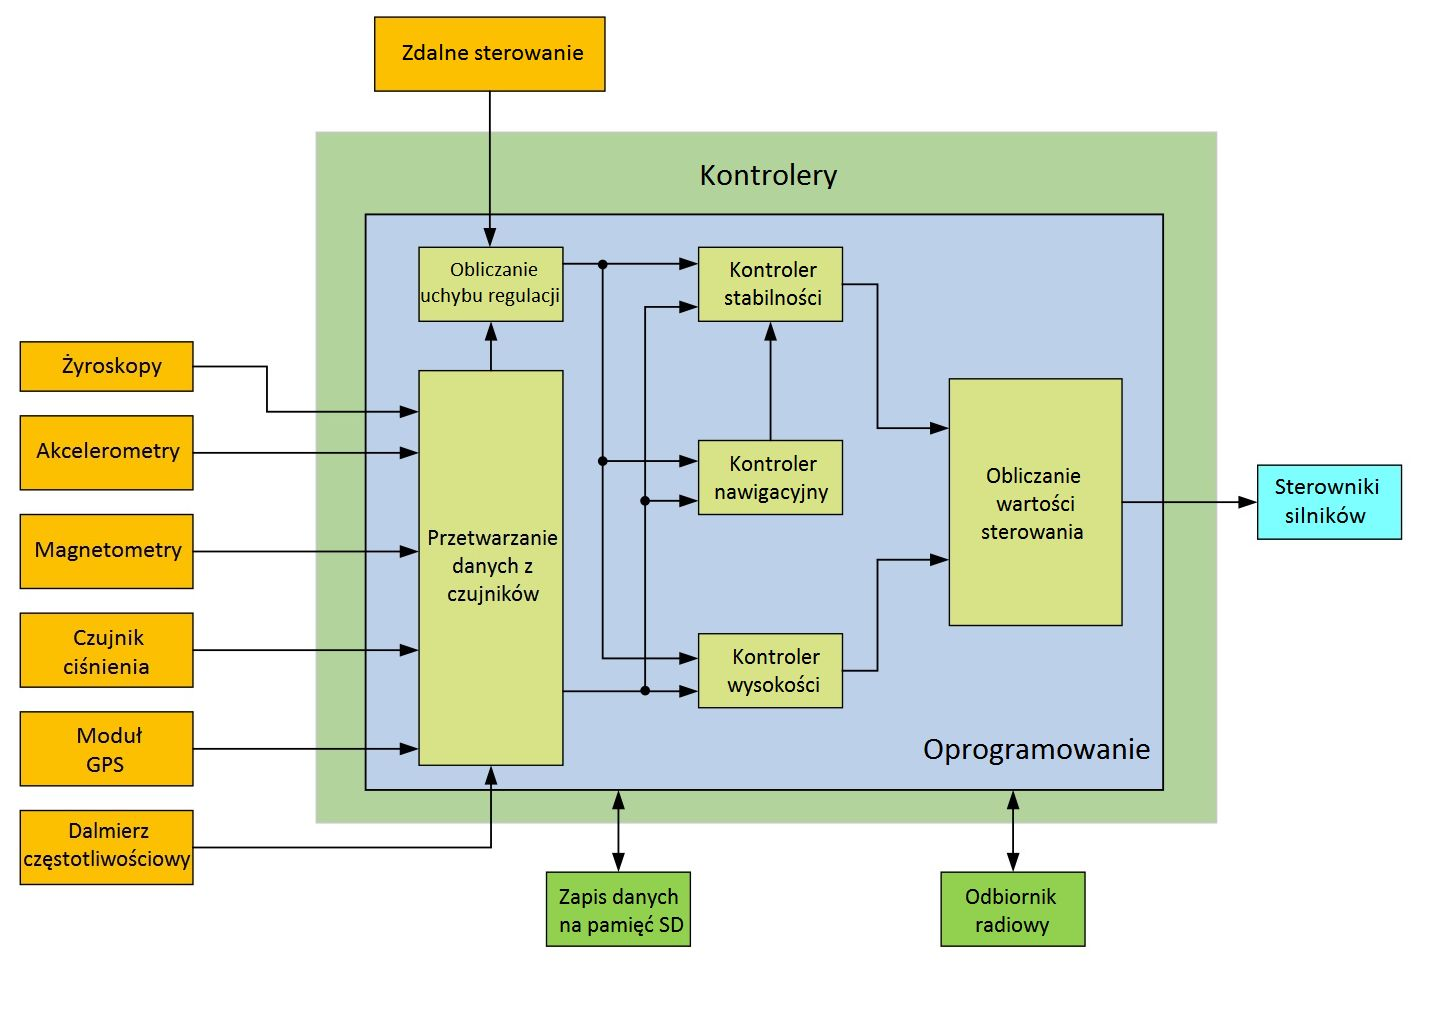
\includegraphics[width=12cm]{7_drone_platform_overview.jpg}
	\caption{Architektura programowo-sprzętowa związana z pracą autopilota \cite{Bouhali2017} }
	\label{fig:autopilot_architecture}
\end{figure} 

Rynek urządzeń typu UAV obfituje w rozwiązania oparte o pracę mikrokontrolerów. Popularnymi autopilotami stosowanymi w komercyjnych produktach -- i przede wszystkim w amatorskich konstrukcjach -- są: NAZA-M V2 firmy DJI oraz Pixhawk firmy 3DR. Oba te moduły, bazując na mikrokontrolerach ARM i dużej liczbie peryferiów, w zupełności wystarczają do zastosowań niewymagających przetwarzania dużej ilości danych, zapewniając łączność z aparaturą radiową i realizację misji opartych na predefiniowanej sekwencji ruchów. 

Nieco bardziej rozbudowane są rozwiązania wykorzystujące dwa mikrokontrolery - jeden z nich jest skonfigurowany w tzw. trybie „baremetal”, który oznacza uruchomienie aplikacji bezpośrednio na procesorze. Umożliwia to wykonywanie niskopoziomowych, krytycznych zadań, a takim z pewnością jest stabilizacja lotu uwzględniająca sterowanie pracą silników i pomiar wartości czujników. Na drugim mikrokontrolerze uruchomiony jest system operacyjny, z poziomu którego działają aplikacje wysokopoziomowe -- takie jak algorytmy planowania trasy, stereowizja czy śledzenie celu. Jedną z takich komercyjnych platform jest „MikroKopter” stworzony przez firmę HiSystems GmbH \cite{MikroKopter}.

\section{Układy rekonfigurowalne w roli autopilota platformy UAV}

Układy rekonfigurowalne, w miarę postępu technologicznego, stają się godną uwagi alternatywą - pomimo często wyższej ceny oferują niezrównanie szybszą prędkość działania algorytmów, jeśli podczas ich implementacji uwzględni się możliwość zrównoleglania obliczeń. 

Przewaga układów rekonfigurowalnych okazuje się być widoczna już w przypadku zadania stabilizacji, a przykładem może być projekt \cite{Eizad}, w którym częstotliwość pracy regulatora PI dla osi obrotu w układzie FPGA osiągała wartość $4.3$MHz, w porównaniu z $0.71$MHz dla rozwiązania programowego na mikrokontrolerze ARM7. Prawdziwym przełomem okazały się być układy SoC, które zintegrowały część procesorową i konfigurowalną, a w efekcie dały sporą swobodę w sposobie realizacji projektu autopilota. Zespół badawczy odpowiedzialny za opisany wyżej projekt wykorzystał układ Zynq w projekcie kolejnego drona, gdzie w części PL zaimplementowano regulację PID, a niezależne podejście programowo-sprzętowe pozwoliło zrealizować algorytm planowania ruchu \cite{Eizad2}. Z kolei dla konstrukcji opisanej w publikacji \cite{Schlender}, najważniejsze zadania rozdzielono pomiędzy 3 procesory w układzie Zynq: 2 z nich, softprocesory Microblaze, odpowiadały za stabilizację, a wyższa warstwa zadań związanych ze zdefiniowaną misją realizowana była w części PS.

Istotnym aspektem pracy autopilota powinna być możliwość zapewnienia odpowiedniego interfejsu komunikacji z szeregiem wykorzystywanych czujników. Układy rekonfigurowalne nie tylko udostępniają ogromną ilość wejść i wyjść, ale są też często wyposażone w sprzętowe kontrolery dla popularnych interfejsów. Ponadto, w przypadku ich niewystarczającej ilości istnieje możliwość sprzętowej implementacji własnego kontrolera. Przede wszystkim jednak, układ rekonfigurowalny pozwala przetworzyć otrzymane wartości w sposób bardziej złożony, niż pozwalałaby na to moc obliczeniowa mikrokontrolera. W publikacji \cite{MEMS} opisano implementację sprzętową cyfrowego kontrolera dla żyroskopów MEMS, który poprzez kwadraturową demodulację sygnału wejściowego i wykorzystanie odpowiednio pętli synchronizacji fazy (PLL) lub automatycznej regulacji wzmocnienia (AGC) poprawia dokładność działania czujnika.

Kolejnym, bardzo ważnym zadaniem autopilota jest estymacja stanu, polegająca na kompensowaniu wszelkich zakłóceń pochodzących z pomiarów. Jest ona najczęściej realizowana w formie filtru Kalmana. Jedna z publikacji \cite{SohKalman} opisuje sprzętowo-programową implementację bezśladowego filtru Kalmana (UKF - Unscented Kalman Filter), której osiągi i zużycie zasobów są konfigurowalne poprzez zdefiniowanie tzw. Bloków Przetwarzania (w liczbach: 1,2,5,10). Algorytm uruchomiony na urządzeniu Zynq XC7Z045 osiągał ponad dwukrotnie większą prędkość działania w porównaniu z rozwiązaniami programowymi i zużywał mniej energii. (131mW dla konfiguracji z pojedynczym Blokiem). 

Ostatnim aspektem pracy autopilota jest generacja sygnałów sterujących silnikami. Na dronach najchętniej montowane są bezszczotkowe silniki prądu stałego, których poprawne działanie wymaga kontrolera sterującego odpowiednim przepływem prądu w uzwojeniach. Zastosowanie układu FPGA pozwala nie tylko generować sygnały PWM wysyłane do kontrolerów prędkości (ESC), ale realizować ich funkcję z pomocą niezależnego obwodu dostarczającego zasilanie. Drugie rozwiązanie zaprezentowano w pracy \cite{ESC}; dzięki niemu osiągnięto wyższą częstotliwości pracy ($12.5$MHz) niż dla tradycyjnego urządzenia ESC ($50$Hz), w efekcie tworząc bardziej responsywną maszynę.

Powyższe rozważania przedstawiają potencjał, jaki osiągnąć mogą autopiloty bazujące na układach rekonfigurowalnych -- jednak jednostki tego typu są już dostępne w sprzedaży. Jedna z nich steruje quadrotorem „Phenox” \cite{Konomura}, w którym część konfigurowalna układu z rodziny Zynq jest odpowiedzialna za przetwarzanie obrazu i dźwięku, generację sygnałów PWM sterujących silnikami i odbiór informacji z czujników.
Kolejny, ważny punkt na osi czasu zaznaczyła firma Aerotenna, która w 2016 roku rozpoczęła produkcję autopilotów kompatybilnych z niezwykle popularnym oprogramowaniem Ardupilot. Pierwszym z urządzeń był „OcPoc”, z układem Zynq-7000 firmy Xilinx. Kilka miesięcy później firma rozszerzyła portfolio o „OcPoC-Cyclone”, którego sercem został układ Intel FPGA Cyclone V \cite{Aerotenna}.

\section{Układy rekonfigurowalne w systemach wizyjnych dla platformy UAV}

Inną grupę rozwiązań stanowią układy realizujące kontrolę wysokiego poziomu, czyli wykorzystanie dodatkowych informacji w celu zapewnienia określonego poziomu autonomiczności.
 
\subsection{Systemy wizyjne bazujące na przetwarzaniu cech}
Jednym z podstawowych sposobów przetwarzania materiału wideo jest ektrakcja jego cech w celu detekcji, klasyfikacji i śledzenia obiektów oraz utrzymywania orientacji kamery. W publikacji \cite{RHOG} porównano dwie grupy algorytmów:
\begin{itemize}
	\item algorytmy detekcji cech: SIFT, FAST, STAR, SURF, ORB, HCD, D-HCD
	\item algorytmy opisu cech: SIFT, FEAK, BRIEF, SURF, ORB, HOG, R-HOG.
\end{itemize} 
Następnie w oparciu o algorytmy D-HCD oraz R-HOG stworzono zintegrowany system w układzie Zynq, który na podstawie analizy cech obrazów pochodzących z dwóch kamer ($1080\times 1920$ @ $30$fps) może być wykorzystany w trójwymiarowym śledzeniu scen, obiektów, multimodalnej rejestracji obrazów lub generowaniu struktur 3D na podstawie ruchu. System z powodzeniem poddano testom na materiałach zarejestrowanych w trakcie lotu, a z zapotrzebowaniem na moc na poziomie $4$W, częstotliwością odświeżania wynoszącą $30$Hz i opóźnieniem poniżej $3$ klatek obrazu, deklasuje laptop z 8-rdzeniowym procesorem Intel i7 2.8GHz, na którym przepustowość uruchomionego algorytmu to zaledwie ok. $2$Hz.

\subsection{Odometria}
Jednym z najprostszych systemów wizyjnych wykorzystywanych przez

\subsection{Systemy stereowizyjne}
Jednym z najczęściej rozważanych systemów wizyjnych wykorzystywanych na plafrormach latających, jest system stereowizyjny. Jego działanie polega na wyznaczeniu współrzędnych punktów sceny trójwymiarowej na podstawie obrazów uzyskiwanych za pomocą co najmniej dwóch kamer, co w efekcie umożliwia określenie odległości od przeszkód lub celów. 
Jednym z rozwiązań tego typu jest \cite{STEREOVISION}. Implementacja algorytmu SGM (Semi-Global Matching) w układzie FPGA (XC7A100T) pozwoliła utworzyć mapę dysparycji w oparciu o obraz o parametrach $480\times 752$ @ $60$fps. Przetworzone dane są przechwytywane przez procesor wykorzystywany zazwyczaj w smartfonach (Samsung Exynos 4412 SoC) i zapisywane w pamięci DDR2. Praca ta została później zresztą wykorzystana na małej platformie UAV \cite{STEREOVISION2}, gdzie spełniała rolę systemu omijania przeszkód o niskiej latencji (poniżej $2$ms).

Kolejnym rozwiązaniem jest system detekcji linii zasilania \cite{STEREOVISION3}. W przypadku małych statków powietrznych, latających zazwyczaj na wysokości kilku-kilkunastu metrów, istnieje zwiększone ryzyko zaczepienia konstrukcją o instalację elektryczną. Opracowany system
wykorzystuje obrazy z dwóch kamer, poddając je równolegle transformacie Censusa oraz transformacji Top-Hat i określając stopień (koszt) dopasowania pomiędzy obrazami. Agregacja kosztów jest obliczana z uwzględnieniem krzyżowego obszaru wsparcia,%cross-based support region
a po nieznacznych ulepszeniach otrzymuje przetworzony obraz z wysegmentowanymi liniami